\documentclass{exam}
\usepackage{../../mypackages}
\usepackage{../../macros}

\title{DST N°2 - Géométrie dans l'espace et Suites}
\author{N. Bancel}
\date{4 Décembre 2024}

\begin{document}

\textbf{Collège Lycée Suger}
\hfill
\textbf{Mathématiques} \\

\textbf{Année 2024-2025}
\hfill
\textbf{1ères STD2A} \par

{\let\newpage\relax\maketitle}

\begin{center}
\textbf{\textcolor{red}{Durée : 2 heures. La calculatrice n'est pas autorisée}} \\
\textbf{\textcolor{red}{Une réponse donnée sans justification sera considérée comme fausse.}} \\
Cette interrogation contient \numquestions\ questions, sur \numpages\ pages et est notée sur 21 points. 

\end{center}

\section*{Exercice 1 : Jeux de rôles (8 points)}

\textbf{Extrait du BAC 2017 STD2A Nouvelle Calédonie} \par
\vspace{1em}
Dans les jeux de rôles, on utilise différents types de dés en plus du classique dé à six faces afin
d'obtenir des résultats différents. Les polyèdres réguliers, connus aussi sous le nom de "solides de
Platon", permettent d'obtenir des dés équiprobables, chaque face ayant la même probabilité de
sortir à chaque tirage. Par exemple, un dé à huit faces a la forme d'un octaèdre régulier.

\subsection*{Étude de l'octaèdre régulier}

Un octaèdre régulier peut-être obtenu à partir d'un cube en prenant pour sommets de l'octaèdre les centres des faces du cube.
On a représenté ci-dessous, en perspective parallèle, un octaèdre régulier ABCDEF inscrit dans un cube dont l'arête mesure 2 cm.
Le point O est le point d'intersection des diagonales du quadrilatère ABCD

\begin{figure}[H]
  \centering
  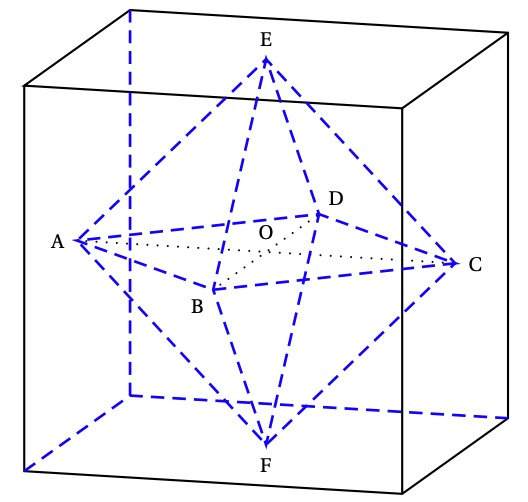
\includegraphics[width=0.4\linewidth]{img/dst_02_01.jpg}
  \caption{\label{} Octaèdre}
\end{figure}

On admet que $\left(O\mathpunct{} ; \ \overrightarrow{OA}\mathpunct{}, \ \overrightarrow{OB}\mathpunct{}, \ \overrightarrow{OE}\right)$ est un repère orthonormal de l'espace.
\begin{questions}
  \question[2.25] Donner les coordonnées des sommets de l'octaèdre régulier ABCDEF dans le repère orthonormal de l'espace $\left(O\mathpunct{} ; \ \overrightarrow{OA}\mathpunct{}, \ \overrightarrow{OB}\mathpunct{}, \ \overrightarrow{OE}\right)$
  \question[1] Que peut-on dire de la sphère de centre O passant par A ?
  \question[1] En utilisant les coordonées de $A$ et de $E$, calculer la longueur AE de l'arête de l'octaèdre régulier ABCD.
  \question[1] Retrouver ce résultat en utilisant le théorème de Pythagore
  \question[1] Calculer les coordonées des vecteurs $\overrightarrow{AE}$ et $\overrightarrow{DF}$
  \question[0.75] En utilisant l'annexe et la question précédente, les droites $(AE)$ et $(DF)$ sont-elles perpendiculaires ? Justifier
  \question[1] Calculer le volume de l'octaèdre régulier ABCDEF. On arrondira le résultat au $cm^3$. On rappelle que le volume $V$ d'une pyramide est donné par la formule :
 \[
  V = \frac{B \times h}{3}
  \]
  où $B$ est l'aire de la base de la pyramide et $h$ la hauteur relative à cette base.
\end{questions} 


\section*{Exercice 2 : Le parallélépipède rectangle (8 points)}

On considère le parallélépipède rectangle $ABCDEFGH$ représenté ci-dessous, tel que $AB = 6$, $AD = 4$ et $AE = 2$.

\begin{center}
    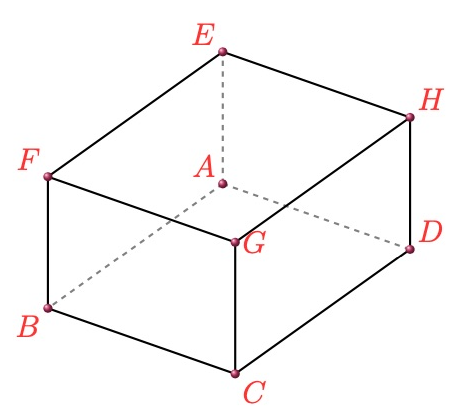
\includegraphics[width=0.5\textwidth]{img/dst_02_02.png}
\end{center}

On se place dans le repère 
\[
\left(A \mathpunct{}; \ \frac{1}{6} \overrightarrow{AB}\mathpunct{}, \ \frac{1}{4} \overrightarrow{AD}\mathpunct{}, \ \frac{1}{2} \overrightarrow{AE}\right).
\]

\begin{questions}
    \question[2] Donner les coordonnées des points $A$, $B$, $C$, $D$, $E$, $F$ et $G$ dans ce repère.

    \question[0.5] Donner les coordonnées du vecteur $\overrightarrow{AC}$.

    \question[0.5] On considère le point $I$ tel que 
    \[
    \overrightarrow{DI} = \frac{1}{2} \overrightarrow{DH}.
    \]
    Placer le point $I$ sur le graphique. Pas besoin de calcul, vous devez pouvoir placer ce point grâce à la compréhension de la notion de vecteur.

    \question[0.5] Donner les coordonnées du point $I$. Bonus : avec une équation (sans utiliser une simple lecture graphique), comment pouvait-on trouver proprement les coordonées du point I ? 

    \question[0.5] En déduire les coordonnées du vecteur $\overrightarrow{EI}$.

    \question[0.5] Soit $J$ le point défini par 
    \[
    \overrightarrow{FJ} = \overrightarrow{FG} + \frac{1}{2} \overrightarrow{GC}.
    \]
    Placer le point $J$ sur le graphique. Pas besoin de calcul, vous devez pouvoir placer ce point grâce à la compréhension de la notion de vecteur.

    \question[0.5] Donner les coordonnées du point $J$. Bonus : avec une équation (sans utiliser une simple lecture graphique), comment pouvait-on trouver proprement les coordonées du point J ? 

    \question[0.5] En déduire les coordonnées du vecteur $\overrightarrow{FJ}$.

    \question[1] Quelle est la nature du quadrilatère $EIFJ$ ? Justifier. (On peut utiliser l'information en annexe pour s'aider à répondre à cette question)

    \question[1] Calculer la longueur des segments $[EF]$ et $[EI]$.

    \question[0.5] En déduire l'aire du quadrilatère $EIFJ$.
\end{questions}


\section*{Exercice 3 : Suites - Exercice identique à celui du BAC Blanc. (5 points)}

\begin{questions}
  \question[2.5] Soit la suite $(U_n)$ définie pour tout $n \geq 0$ par la relation suivante :
  
  \[
    \left\{
      \begin{array}{ll}
            U_{n+1} = U_n + n \\
            U_0 = 2 
        \end{array}
      \right.
    \]
  
  \begin{parts}
    \part[1] Calculer les trois premiers termes de la suite $(U_n)$.
    \part[1] Calculer $U_{n+1} - U_{n}$
    \part[0.5] Cette suite est-elle croissante ou décroissante ? Justifier
  \end{parts}

  \question[2.5] Soit la suite \((V_n)\) définie par la relation fonctionnelle :
  \[
  V_n = 5 \times 2^n.
  \]
  \begin{parts}
    \part[1] Calculer les termes $V_0$, $V_1$ et $V_2$.
    \part[1] Calculer le rapport $\frac{V_{n+1}}{V_n}$
    \part[0.5] Déterminer si la suite $(V_n)$ est géométrique, et préciser sa raison. Cette suite est-elle croissante ou décroissante ? Justifier
  \end{parts}

\end{questions}

\section*{Annexe}

\begin{itemize}
  \item Un polygone est régulier si et seulement si tous ses côtés ont la même longueur
  \item On peut dire que deux droites sont parallèles si et seulement si leurs vecteurs directeurs (les vecteurs qui suivent la direction de la droite) sont colinéaires.
  \item On dit que 2 vecteurs $\overrightarrow{AB}$ et $\overrightarrow{CD}$ respectivement de coordonées $x_{AB}, y_{AB}, z_{AB}$ et $x_{CD}, y_{CD}, z_{CD}$ sont colinéires si et seulement si on peut écrire 
  \[
  \overrightarrow{AB} = \alpha \cdot \overrightarrow{CD}
  \]
 c'est-à-dire
  \[
  \begin{pmatrix}
    x_{AB} \\
    y_{AB} \\ 
    z_{AB}
  \end{pmatrix}
  = 
  \alpha \cdot
  \begin{pmatrix}
    x_{CD} \\
    y_{CD} \\ 
    z_{CD}
  \end{pmatrix}
\] 
autrement dit 
\[
  \begin{pmatrix}
    x_{AB} \\
    y_{AB} \\ 
    z_{AB}
  \end{pmatrix}
  =
  \begin{pmatrix}
    \alpha \cdot x_{CD} \\
    \alpha \cdot y_{CD} \\ 
    \alpha \cdot z_{CD}
  \end{pmatrix}
\] 
\item Soit A, B, C et D quatre points du plan. Les droites (AB) et (CD) sont perpendiculaires si et seulement si les vecteurs $\overrightarrow{AB}$ et $\overrightarrow{CD}$ sont orthogonaux.
\item Deux vecteurs $\overrightarrow{AB}$ et $\overrightarrow{CD}$ de coordonnées \\ 

\[
  \overrightarrow{AB} = 
  \begin{pmatrix}
    x_{AB} \\
    y_{AB} \\ 
    z_{AB}
  \end{pmatrix}
\] et
\[
  \overrightarrow{CD} = 
  \begin{pmatrix}
    x_{CD} \\
    y_{CD} \\ 
    z_{CD}
  \end{pmatrix}
\]
sont orthogonaux si et seulement si leur produit scalaire est égal à 0, c'est-à-dire : 
\[
  x_{AB} \cdot x_{CD} + y_{AB} \cdot y_{CD} + z_{AB} \cdot z_{CD} = 0
\]
\end{itemize}




\end{document}
